\chapter{Double Descent with Random Projections}
\label{ch:double-descent}

\section{Motivation}
\label{sec:3.1}

One of the central puzzles in deep learning is the following: modern neural networks are often heavily overparameterized, so in principle they can interpolate (and even memorize) the training data, yet in practice they can still generalize well on unseen data. This tension between expressive power and test performance motivated a large line of work on the interpolation regime. Double descent is a first clean window into this phenomenon \cite{belkin2019reconciling}: in overparameterized linear and random-feature models, it shows explicitly how prediction risk can worsen near interpolation and then improve again beyond it, offering a concrete baseline mechanism for why ``more parameters'' need not imply worse generalization.

An illustrative non-isotropic example is shown in Figure~\ref{fig:3.1}, where the risk first decreases, spikes near interpolation, and then decreases again.

A tractable way to study this behavior is through a random-feature model: the weights defining the hidden features are sampled once and then frozen, while only the readout coefficients are fitted by least squares. Conditional on the frozen features, training is therefore linear regression. We specialize to a linear activation, for which the feature matrix is a random projection of the input matrix.

Although simple, this model retains the rank mechanisms behind double descent. If the ambient dimension exceeds the sample size, increasing the number of random features crosses an interpolation threshold; if the ambient dimension is smaller, the random features eventually span the input space and further increases in width do not change the fitted function. In the isotropic Gaussian setting, rotational invariance gives explicit bias--variance formulas across these rank regimes. Bach's general-covariance analysis is our starting point \cite{bach2024high}.

\begin{figure}[t]
\centering
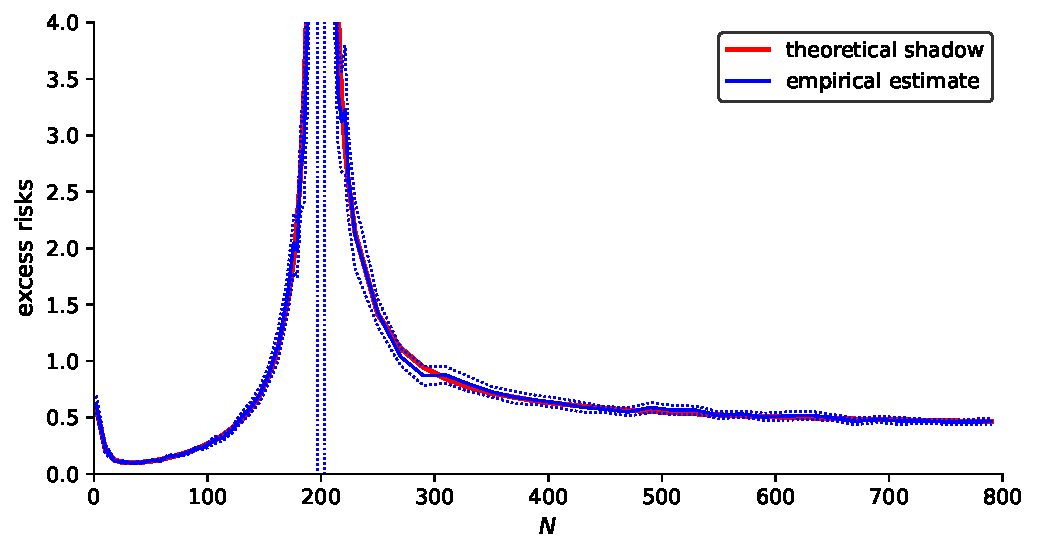
\includegraphics[width=0.82\textwidth]{figures/fig3_1_double_descent.pdf}
\caption{A non-isotropic double descent example for linear regression with random projections, with $m = 200$ observations and ambient dimension $n_0 = 400$. Adapted from \cite[Figure~1]{bach2024high}; the horizontal axis has been relabeled by $n$, the finite-dimensional counterpart of our notation $N$ for the number of random projections. The isotropic model below exhibits the interpolation spike and second descent when the ambient dimension exceeds the sample size, but not the initial descent visible here.}
\label{fig:3.1}
\end{figure}

\section{Model: Linear Regression with Random Projections}
\label{sec:3.2}

Working at internal dimensions $M, N_0, N \in \hN$ (extending finite dimensions $(m, n_0, n) \in \N^3$ by the Transfer Principle), we observe
\begin{equation}\label{eq:3.1}
y = X\theta_\star + \varepsilon, \qquad X \in \hR^{M \times N_0}, \quad X_{ij} \stackrel{\mathrm{iid}}{\sim} \hNcal(0, 1), \qquad \varepsilon \sim \hNcal(0, \sigma^2 I_M),
\end{equation}
where $\theta_\star \in \hR^{N_0}$ is the unknown internal parameter, $\sigma^2 \in \R_{\ge 0}$ is the noise variance, and $X$ is internally independent of $\varepsilon$. Let $S \in \hR^{N_0 \times N}$ be an internal random projection matrix with i.i.d.\ entries
\begin{equation}\label{eq:3.2}
S_{jk} \stackrel{\mathrm{iid}}{\sim} \hNcal(0, 1), \qquad S \text{ internally independent of } (X, \varepsilon).
\end{equation}
We fit a linear predictor in the projected feature space $x \mapsto S^\top x$. The projected design matrix, minimum-norm feature coefficient, and induced ambient coefficient are
\begin{equation}\label{eq:3.3}
Z := XS \in \hR^{M \times N}, \qquad \hat{\eta} := Z^\dagger y = \bigl(Z^\top Z\bigr)^\dagger Z^\top y \in \hR^N, \qquad \hat{\theta} := S\hat{\eta} \in \hR^{N_0},
\end{equation}
where $\dagger$ denotes the internal Moore--Penrose pseudoinverse, obtained by Transfer of the finite-dimensional pseudoinverse.

Thus $M$, $N_0$, and $N$ (with finite-dimensional counterparts $m$, $n_0$, and $n$ in Figure~\ref{fig:3.1}) denote the number of observations, the ambient dimension, and the number of random projections, respectively. This differs from Bach's notation: there, $n$ denotes the number of observations, $m$ the number of random projections, and $d$ the ambient dimension \cite{bach2024high}.

We measure parameter estimation error by the internal squared Euclidean norm
\begin{equation}\label{eq:3.4}
R(\hat{\theta}) := \norm{\hat{\theta} - \theta_\star}^2.
\end{equation}
For an internally independent test covariate $x_{\mathrm{new}} \sim \hNcal(0, I_{N_0})$, Transfer shows that this also equals the internal excess prediction error $\hE_{x_{\mathrm{new}}}\bigl[(x_{\mathrm{new}}^\top(\hat{\theta} - \theta_\star))^2\bigr]$. For a general internal covariance $\Sigma = \hE[xx^\top]$, prediction error instead equals $(\hat{\theta} - \theta_\star)^\top \Sigma (\hat{\theta} - \theta_\star)$ and need not coincide with $R(\hat{\theta})$. Since $\hat{\theta} = \mathcal{M}y$ for the internal linear estimator map
\begin{equation}\label{eq:3.5}
\mathcal{M} := SZ^\dagger = S\bigl(Z^\top Z\bigr)^\dagger Z^\top,
\end{equation}
substituting $y = X\theta_\star + \varepsilon$ gives, by Transfer of the finite-dimensional bias--variance identity, the exact internal bias--variance decomposition
\begin{equation}\label{eq:3.6}
\hE_\varepsilon\bigl[R(\hat{\theta}) \;\big|\; X, S\bigr] = \norm{(\mathcal{M}X - I_{N_0})\theta_\star}^2 + \hE_\varepsilon\norm{\mathcal{M}\varepsilon}^2 = R^{(\mathrm{bias})}(\hat{\theta}) + R^{(\mathrm{var})}(\hat{\theta}),
\end{equation}
where
\begin{equation}\label{eq:3.7}
R^{(\mathrm{var})}(\hat{\theta}) = \sigma^2 \Tr\bigl(\mathcal{M}^\top \mathcal{M}\bigr).
\end{equation}

\section{High-Dimensional Risk and Double Descent}
\label{sec:3.3}

We now state the standard shadow behavior of the internal conditional risk $\hE_\varepsilon\bigl[R(\hat{\theta}) \;\big|\; X, S\bigr]$ (equivalently the internal conditional bias--variance terms from \eqref{eq:3.6}) for unlimited dimensions in the proportional galaxy
\begin{equation}\label{eq:3.8}
M, N_0, N \in \hNinf \qquad \text{with} \qquad \gamma := \st\!\left(\frac{N_0}{M}\right) \in (0, \infty), \qquad \delta := \st\!\left(\frac{N}{M}\right) \in (0, \infty).
\end{equation}
Recall that for internal random variables $U, V$ on the joint probability space of $(X, S)$, the notation $U \approxP V$ means that $U \approx V$ holds $\Loeb$-almost surely (equivalently, $\st\bigl(\hP(\abs{U - V} > \epsilon)\bigr) = 0$ for every standard $\epsilon > 0$).

The following theorem gives the three rank regimes for the Gaussian isotropic model. The feature- and sample-bottleneck formulas are the $\Sigma = I_{N_0}$ specialization of \cite[Proposition~4]{bach2024high}; the ambient-bottleneck formula follows directly from internal ordinary least squares once the random features span $\hR^{N_0}$.

\begin{theorem}[Asymptotic Bias and Variance for Random Projections (Isotropic Case)]\label{thm:3.1}
Assume the internal isotropic Gaussian model \eqref{eq:3.1}--\eqref{eq:3.2} and consider the ridgeless estimator \eqref{eq:3.3}. In the proportional galaxy \eqref{eq:3.8}, assume that $\theta_\star \in \hR^{N_0}$ satisfies $\norm{\theta_\star}^2 \in \Lim$ with standard shadow $\st\bigl(\norm{\theta_\star}^2\bigr) \in [0, \infty)$. Then, in each of the following regimes, the internal conditional bias--variance terms in \eqref{eq:3.6} concentrate infinitesimally in Loeb probability $\Loeb$, with respect to the randomness of $(X, S)$, around the displayed deterministic standard values.
\begin{enumerate}[label=(\alph*)]
\item \emph{Feature-bottleneck regime} ($\delta < \min\{1, \gamma\}$):
\begin{align}
R^{(\mathrm{var})}(\hat{\theta}) &\approxP \sigma^2 \frac{\delta}{1 - \delta}, \label{eq:3.9} \\
R^{(\mathrm{bias})}(\hat{\theta}) &\approxP \frac{\gamma - \delta}{\gamma(1 - \delta)} \st\bigl(\norm{\theta_\star}^2\bigr). \label{eq:3.10}
\end{align}

\item \emph{Ambient-bottleneck regime} ($\gamma < 1$ and $\delta \ge \gamma$):
\begin{align}
R^{(\mathrm{var})}(\hat{\theta}) &\approxP \sigma^2 \frac{\gamma}{1 - \gamma}, \label{eq:3.11} \\
R^{(\mathrm{bias})}(\hat{\theta}) &\approxP 0. \label{eq:3.12}
\end{align}

\item \emph{Sample-bottleneck regime} ($\gamma > 1$ and $\delta > 1$):
\begin{align}
R^{(\mathrm{var})}(\hat{\theta}) &\approxP \sigma^2\!\left(\frac{1}{\gamma - 1} + \frac{1}{\delta - 1}\right), \label{eq:3.13} \\
R^{(\mathrm{bias})}(\hat{\theta}) &\approxP \left(1 - \frac{1}{\gamma}\right)\frac{\delta}{\delta - 1} \st\bigl(\norm{\theta_\star}^2\bigr). \label{eq:3.14}
\end{align}
\end{enumerate}
The theorem excludes the singular boundaries $\delta = 1$ for $\gamma > 1$ and $\gamma = 1$ for $\delta \ge 1$.
\end{theorem}

The theorem is most easily read by fixing $\gamma$ and increasing the width ratio $\delta$. When $\gamma > 1$, the feature-bottleneck formulas apply for $\delta < 1$, up to the boundary. Provided $\sigma^2 > 0$ or the standard shadow $\st\bigl(\norm{\theta_\star}^2\bigr)$ is positive, the standard total risk is strictly increasing and diverges as $\delta \uparrow 1$. The closing dimension gap $M - N$ makes the random design nearly square relative to $M$ and produces the interpolation spike. For $\delta > 1$, the sample-bottleneck formulas apply, and the part of the risk shadow above its large-$\delta$ asymptote decreases proportionally to $(\delta - 1)^{-1}$ toward $\sigma^2/(\gamma - 1) + (1 - 1/\gamma)\st\bigl(\norm{\theta_\star}^2\bigr)$ as $\delta \to \infty$. This is the second descent. Thus the isotropic model captures the interpolation spike and the post-interpolation descent, but not the initial descent in Figure~\ref{fig:3.1}.

When $\gamma < 1$, the width ratio reaches the ambient dimension ratio first, at $\delta = \gamma < 1$. The feature-bottleneck formulas then meet the ambient-bottleneck formulas continuously: the bias shadow vanishes, and the risk shadow remains at the ordinary least-squares value $\sigma^2\gamma/(1 - \gamma)$ for all $\delta \ge \gamma$. Consequently there is no singularity at $\delta = 1$; before ambient saturation, the risk shadow may increase, decrease, or remain flat depending on the signal-to-noise ratio. In this way, $\gamma$ determines whether increasing width first reaches the interpolation threshold or the ambient dimension, while $\delta$ determines the active bottleneck.

\subsection{Gaussian Derivation of the Risk Theorem}
\label{sec:3.3.1}

We now give the nonstandard derivation behind each branch of Theorem~\ref{thm:3.1}. By the Transfer Principle, every finite-dimensional linear-algebra identity and conditional Gaussian expectation holds verbatim at hyperfinite dimensions $(M, N_0, N)$. In the strict proportional regimes, strict standard inequalities on $(\gamma, \delta)$ immediately enforce the corresponding internal rank inequalities on $(M, N_0, N)$, and infinitesimal variance bounds upgrade the internal conditional-mean formulas to $\Loeb$-concentration of the random risk terms around their standard shadows.

\begin{lemma}[Gaussian Gram-Matrix Inputs]\label{lem:3.2}
Let $P, Q \in \hN$ and let $G \in \hR^{P \times Q}$ have i.i.d.\ $\hNcal(0, 1)$ entries. The internal inverse-Wishart identities are
\begin{equation}\label{eq:3.15}
\hE\bigl[(G^\top G)^{-1}\bigr] = \frac{I_Q}{P - Q - 1}, \quad P > Q + 1, \qquad \hE\bigl[(G G^\top)^{-1}\bigr] = \frac{I_P}{Q - P - 1}, \quad Q > P + 1.
\end{equation}
Consequently, for $P, Q \in \hNinf$ away from the square boundary $\st(Q/P) = 1$,
\begin{equation}\label{eq:3.16}
\Tr\bigl((G^\top G)^{-1}\bigr) \approxP \frac{\rho}{1 - \rho}, \; \st\!\left(\frac{Q}{P}\right) = \rho < 1, \quad \Tr\bigl((G G^\top)^{-1}\bigr) \approxP \frac{1}{\rho - 1}, \; \st\!\left(\frac{Q}{P}\right) = \rho > 1.
\end{equation}
\end{lemma}

\begin{proof}
The identities in \eqref{eq:3.15} hold verbatim for all hyperintegers $P, Q \in \hN$ by Transfer of the standard first inverse moments of a finite-dimensional Wishart matrix. When $P, Q \in \hNinf$ satisfy $\st(Q/P) = \rho < 1$ (respectively, $\st(Q/P) = \rho > 1$), we immediately have $P > Q + 3$ (respectively, $Q > P + 3$), and the transferred inverse-Wishart trace variance is infinitesimal, so internal Chebyshev concentration yields $\Tr\bigl((G^\top G)^{-1}\bigr) \approxP Q/(P - Q - 1) \approx \rho/(1 - \rho)$ (respectively, $\Tr\bigl((G G^\top)^{-1}\bigr) \approxP P/(Q - P - 1) \approx 1/(\rho - 1)$).
\end{proof}

\begin{lemma}[Directional Inverse-Wishart Law]\label{lem:3.3}
If $P, Q \in \hN$ satisfy $Q > P$, $G \in \hR^{P \times Q}$ has i.i.d.\ $\hNcal(0, 1)$ entries, and $a \in \hR^P$ is internally deterministic, then
\begin{equation}\label{eq:3.17}
a^\top (G G^\top)^{-1} a \eqd \frac{\norm{a}^2}{\ns{\chi}^2_{Q - P + 1}}
\end{equation}
in internal law under $\hP$, with the zero-vector case interpreted directly.
\end{lemma}

\begin{proof}
By Transfer of the finite-dimensional directional calculation, for $a \neq 0$ internal orthogonal invariance reduces to $a = \norm{a}e_1$. Writing the first row of $G$ as $g_1$ and the remaining rows as $G_2$, the transferred Schur-complement identity gives
\begin{equation}\label{eq:3.18}
\bigl[(G G^\top)^{-1}\bigr]_{11}^{-1} = g_1\bigl(I_Q - G_2^\top(G_2 G_2^\top)^{-1}G_2\bigr)g_1^\top.
\end{equation}
The matrix in parentheses is an internal orthogonal projector of hyperfinite rank $Q - P + 1$, internally independent of $g_1$, so by Transfer the right-hand side has the internal $\ns{\chi}^2_{Q - P + 1}$ distribution.
\end{proof}

\begin{lemma}[Haar Projection Lengths]\label{lem:3.4}
Let $D_0, K \in \hN$ satisfy $K \le D_0$, and let $P$ be the internal orthogonal projector onto an internally Haar-distributed $K$-dimensional subspace of $\hR^{D_0}$. For every internally deterministic $v \in \hR^{D_0}$,
\begin{equation}\label{eq:3.19}
\hE\bigl[\norm{Pv}^2\bigr] = \frac{K}{D_0}\norm{v}^2.
\end{equation}
If $D_0 \in \hNinf$ and $\st(K / D_0) = \rho \in [0, 1]$, then $\norm{Pv}^2 - (K / D_0)\norm{v}^2 \approxP 0$ for every internally deterministic $v \in \hR^{D_0}$ with $\norm{v}^2 \in \Lim$.
\end{lemma}

\begin{proof}
For $v = 0$, both conclusions are immediate, so suppose $v \neq 0$. By Transfer, rotating $v$ to the first coordinate and representing an internally uniform direction by a normalized $\hNcal(0, I_{D_0})$ vector shows that $\norm{Pv}^2 / \norm{v}^2$ has the same internal law as $\ns{\chi}^2_K / (\ns{\chi}^2_K + \widetilde{\ns{\chi}}^2_{D_0 - K})$, where the two internal chi-squared variables are internally independent. The internal mean \eqref{eq:3.19} follows by symmetry. If $\rho \in (0, 1)$, both $K$ and $D_0 - K$ belong to $\hNinf$, so internal Chebyshev concentration gives $\ns{\chi}^2_K / D_0 \approxP \rho$ and $\widetilde{\ns{\chi}}^2_{D_0 - K} / D_0 \approxP 1 - \rho$, whence $\norm{Pv}^2 / \norm{v}^2 \approxP \rho \approx K / D_0$. If $\rho = 0$, the claim follows from the mean identity \eqref{eq:3.19} and internal Markov's inequality; if $\rho = 1$, apply the same argument to $I_{D_0} - P$. Multiplying by $\norm{v}^2 \in \Lim$ yields $\norm{Pv}^2 - (K / D_0)\norm{v}^2 \approxP 0$.
\end{proof}

All infinitesimal concentration statements $\approxP$ below refer to the Loeb probability space $\Loeb$ of the joint randomness of $(X, S)$. The intermediate internal conditional expectations are proof devices and are distinct from the label-noise expectation in \eqref{eq:3.6}.

\begin{proposition}[Feature-Bottleneck Calculation]\label{prop:3.5}
Under the assumptions of Theorem~\ref{thm:3.1}, if $\delta < \min\{1, \gamma\}$, then
\begin{equation}\label{eq:3.20}
R^{(\mathrm{var})}(\hat{\theta}) \approxP \sigma^2 \frac{\delta}{1 - \delta}, \qquad R^{(\mathrm{bias})}(\hat{\theta}) \approxP \frac{\gamma - \delta}{\gamma(1 - \delta)} \st\bigl(\norm{\theta_\star}^2\bigr).
\end{equation}
\end{proposition}

\begin{proof}
Since $\st(N / M) = \delta < 1$ and $\st(N / N_0) = \delta / \gamma < 1$, the strict standard inequalities immediately imply $N < \min\{M, N_0\}$. By Transfer, write the internal thin QR factorization
\begin{equation}\label{eq:3.21}
S = QT, \qquad Q^\top Q = I_N,
\end{equation}
where $T \in \hR^{N \times N}$ is invertible $\hP$-almost surely. Since $Z = (XQ)T$ has full column rank $N$, Transfer gives for the least-squares coefficient and its mapped ambient parameter the exact internal identities
\begin{equation}\label{eq:3.22}
\begin{aligned}
\hat{\eta} &= \bigl(T^\top (XQ)^\top (XQ) T\bigr)^{-1} T^\top (XQ)^\top y = T^{-1}\bigl((XQ)^\top XQ\bigr)^{-1}(XQ)^\top y, \\
\hat{\theta} &= Q\bigl((XQ)^\top XQ\bigr)^{-1}(XQ)^\top y.
\end{aligned}
\end{equation}
Thus the internal singular values of $S$ cancel: in this regime the mapped estimator $\hat{\theta}$ depends on $S$ only through its column space.

Set
\begin{equation}\label{eq:3.23}
P_S := QQ^\top, \qquad \theta_\perp := (I_{N_0} - P_S)\theta_\star.
\end{equation}
The response decomposes internally as
\begin{equation}\label{eq:3.24}
y = (XQ)Q^\top \theta_\star + X\theta_\perp + \varepsilon.
\end{equation}
Internally conditional on $Q$, the matrix $XQ$ has i.i.d.\ $\hNcal(0, 1)$ entries and $X\theta_\perp$ is internally independent of $XQ$, with internal distribution $\hNcal(0, \norm{\theta_\perp}^2 I_M)$. Substituting \eqref{eq:3.24} into \eqref{eq:3.22} gives
\begin{equation}\label{eq:3.25}
\hat{\theta} = P_S\theta_\star + Q\bigl((XQ)^\top XQ\bigr)^{-1}(XQ)^\top X\theta_\perp + Q\bigl((XQ)^\top XQ\bigr)^{-1}(XQ)^\top \varepsilon.
\end{equation}
The last term is the label-noise contribution. Using $Q^\top Q = I_N$ and internal cyclicity of trace, its conditional variance is
\begin{equation}\label{eq:3.26}
R^{(\mathrm{var})}(\hat{\theta}) = \sigma^2 \Tr\Bigl[(XQ)\bigl((XQ)^\top XQ\bigr)^{-2}(XQ)^\top\Bigr] = \sigma^2 \Tr\Bigl[\bigl((XQ)^\top XQ\bigr)^{-1}\Bigr].
\end{equation}
After averaging internally only over the label noise and subtracting $\theta_\star$, the bias vector is $-\theta_\perp + Q((XQ)^\top XQ)^{-1}(XQ)^\top X\theta_\perp$. These two terms lie in the internally orthogonal subspaces $\spn(Q)^\perp$ and $\spn(Q)$, respectively, so the conditional squared bias is exactly
\begin{equation}\label{eq:3.27}
R^{(\mathrm{bias})}(\hat{\theta}) = \norm{\theta_\perp}^2 + (X\theta_\perp)^\top (XQ)\bigl((XQ)^\top XQ\bigr)^{-2}(XQ)^\top X\theta_\perp.
\end{equation}
Internally conditional on $(Q, XQ)$, the expectation of the second term over the independent internal Gaussian vector $X\theta_\perp$ is
\begin{equation}\label{eq:3.28}
\hE\Bigl[(X\theta_\perp)^\top (XQ)\bigl((XQ)^\top XQ\bigr)^{-2}(XQ)^\top X\theta_\perp \;\Big|\; Q, XQ\Bigr] = \norm{\theta_\perp}^2 \Tr\Bigl[\bigl((XQ)^\top XQ\bigr)^{-1}\Bigr],
\end{equation}
while its internal conditional variance $2\norm{\theta_\perp}^4 \Tr\bigl(((XQ)^\top XQ)^{-2}\bigr)$ is infinitesimal since $\norm{\theta_\perp}^2 \le \norm{\theta_\star}^2 \in \Lim$ and $\hE\bigl[\Tr(((XQ)^\top XQ)^{-2})\bigr] = O(1/M) \in \Inf$. Internal Gaussian quadratic-form concentration therefore yields
\begin{equation}\label{eq:3.29}
R^{(\mathrm{bias})}(\hat{\theta}) \approxP \norm{\theta_\perp}^2 \Bigl[1 + \Tr\bigl(((XQ)^\top XQ)^{-1}\bigr)\Bigr].
\end{equation}
By Transfer, the exact fully averaged internal identities provide a hyperfinite check:
\begin{equation}\label{eq:3.30}
\hE_{X, S}\bigl[R^{(\mathrm{var})}(\hat{\theta})\bigr] = \sigma^2 \frac{N}{M - N - 1}, \qquad \hE_{X, S}\bigl[R^{(\mathrm{bias})}(\hat{\theta})\bigr] = \left(1 - \frac{N}{N_0}\right)\frac{M - 1}{M - N - 1}\norm{\theta_\star}^2,
\end{equation}
whenever $N \le N_0$ and $M > N + 1$. Indeed, \eqref{eq:3.19} gives the omitted-signal factor $1 - N / N_0$, while \eqref{eq:3.15} gives the amplification factor $1 + N / (M - N - 1) = (M - 1) / (M - N - 1)$.

Here $XQ \in \hR^{M \times N}$ has i.i.d.\ $\hNcal(0, 1)$ entries, while $I_{N_0} - P_S$ projects onto an internally Haar-distributed $(N_0 - N)$-dimensional subspace of $\hR^{N_0}$. Since $\st(N / M) = \delta$ and $\st((N_0 - N) / N_0) = 1 - \delta / \gamma$, applying Lemmas~\ref{lem:3.2} and~\ref{lem:3.4} gives
\begin{equation}\label{eq:3.31}
\Tr\bigl(((XQ)^\top XQ)^{-1}\bigr) \approxP \frac{\delta}{1 - \delta}, \qquad \norm{\theta_\perp}^2 \approxP \left(1 - \frac{\delta}{\gamma}\right)\st\bigl(\norm{\theta_\star}^2\bigr).
\end{equation}
The first concentration relation in \eqref{eq:3.31}, combined with \eqref{eq:3.26}, gives the variance shadow in \eqref{eq:3.20}. Since $1 + \delta / (1 - \delta) = (1 - \delta)^{-1}$, substitution in \eqref{eq:3.29} gives the bias shadow. The same inverse-Wishart factor therefore amplifies both label noise and the omitted signal.
\end{proof}

\begin{proposition}[Ambient-Bottleneck Calculation]\label{prop:3.6}
Under the assumptions of Theorem~\ref{thm:3.1}, if $\gamma < 1$ and $\delta > \gamma$, then
\begin{equation}\label{eq:3.32}
R^{(\mathrm{var})}(\hat{\theta}) \approxP \sigma^2 \frac{\gamma}{1 - \gamma}, \qquad R^{(\mathrm{bias})}(\hat{\theta}) \approxP 0.
\end{equation}
\end{proposition}

\begin{proof}
Since $\st(N_0 / M) = \gamma < 1$ and $\st(N / M) = \delta > \gamma$, we immediately have the internal inequalities $N_0 < M$ and $N > N_0$ (in particular $N \ge N_0$). By Transfer, the matrices $X$ and $S$ then have full column rank $N_0$ and full row rank $N_0$, respectively, $\hP$-almost surely. By Transfer, the least-squares coefficient $\hat{\eta} = Z^\dagger y$ satisfies the internal normal equations
\begin{equation}\label{eq:3.33}
S^\top X^\top (XS\hat{\eta} - y) = 0.
\end{equation}
Because $S^\top$ is internally injective and $\hat{\theta} = S\hat{\eta}$, these equations imply
\begin{equation}\label{eq:3.34}
X^\top\bigl(X\hat{\theta} - y\bigr) = 0, \qquad \hat{\theta} = (X^\top X)^{-1} X^\top y.
\end{equation}
Thus the particular minimum-feature-norm solution maps to the unique ambient internal ordinary least-squares solution. Substituting the model gives
\begin{equation}\label{eq:3.35}
\hat{\theta} - \theta_\star = (X^\top X)^{-1} X^\top \varepsilon.
\end{equation}
Hence the internal conditional bias vanishes identically ($R^{(\mathrm{bias})}(\hat{\theta}) = 0$) and
\begin{equation}\label{eq:3.36}
R^{(\mathrm{var})}(\hat{\theta}) = \sigma^2 \Tr\bigl((X^\top X)^{-1} X^\top X (X^\top X)^{-1}\bigr) = \sigma^2 \Tr\bigl((X^\top X)^{-1}\bigr).
\end{equation}
In particular, by \eqref{eq:3.15},
\begin{equation}\label{eq:3.37}
\hE_X\bigl[R^{(\mathrm{var})}(\hat{\theta})\bigr] = \sigma^2 \frac{N_0}{M - N_0 - 1},
\end{equation}
whenever $M > N_0 + 1$. The tall-matrix case of Lemma~\ref{lem:3.2} now gives $R^{(\mathrm{var})}(\hat{\theta}) \approxP \sigma^2 \gamma / (1 - \gamma)$, proving \eqref{eq:3.32}.
\end{proof}

\begin{lemma}[Gaussian Row--Null Coordinates]\label{lem:3.7}
Suppose $M < N_0$ and $X \in \hR^{M \times N_0}$ has full row rank, with $S$ internally independent of $X$ and distributed as in \eqref{eq:3.2}. Set $U_X := X^\top (X X^\top)^{-1/2}$ and choose an internal matrix $U_\perp \in \hR^{N_0 \times (N_0 - M)}$ with orthonormal columns spanning $\ker(X)$. Internally conditional on $X$, the matrices $H := U_X^\top S$ and $G_\perp := U_\perp^\top S$ are internally independent standard Gaussian matrices with i.i.d.\ $\hNcal(0, 1)$ entries.
\end{lemma}

\begin{proof}
By Transfer, $U_X$ has orthonormal columns and is orthogonal to $U_\perp$. Indeed,
\begin{equation}\label{eq:3.38}
[U_X \;\; U_\perp]^\top [U_X \;\; U_\perp] = I_{N_0},
\end{equation}
so $[U_X \;\; U_\perp]$ is internally orthogonal. Internally conditional on $X$, applying its transpose to each $\hNcal(0, I_{N_0})$ column of $S$ gives internally independent standard Gaussian row and null coordinates.
\end{proof}

\begin{proposition}[Sample-Bottleneck Calculation]\label{prop:3.8}
Under the assumptions of Theorem~\ref{thm:3.1}, if $\gamma > 1$ and $\delta > 1$, then
\begin{equation}\label{eq:3.39}
R^{(\mathrm{var})}(\hat{\theta}) \approxP \sigma^2\!\left(\frac{1}{\gamma - 1} + \frac{1}{\delta - 1}\right), \qquad R^{(\mathrm{bias})}(\hat{\theta}) \approxP \left(1 - \frac{1}{\gamma}\right)\frac{\delta}{\delta - 1} \st\bigl(\norm{\theta_\star}^2\bigr).
\end{equation}
\end{proposition}

\begin{proof}
Since $\st(N_0 / M) = \gamma > 1$ and $\st(N / M) = \delta > 1$, the strict standard inequalities immediately give $M < \min\{N_0, N\}$, so $Z$ has full row rank $M$ $\hP$-almost surely and, by Transfer,
\begin{equation}\label{eq:3.40}
Z^\dagger = Z^\top (Z Z^\top)^{-1}.
\end{equation}
Use the internal matrices $U_X, U_\perp, H, G_\perp$ from Lemma~\ref{lem:3.7}. Since $[U_X \;\; U_\perp]$ is internally orthogonal and $H = (X X^\top)^{-1/2}Z$, projecting $S$ onto these two coordinate blocks gives
\begin{equation}\label{eq:3.41}
S = X^\top (X X^\top)^{-1} Z + U_\perp G_\perp, \qquad Z = (X X^\top)^{1/2} H.
\end{equation}
Substituting \eqref{eq:3.41} into $\mathcal{M} = S Z^\dagger$ and using $Z Z^\dagger = I_M$ gives
\begin{equation}\label{eq:3.42}
\mathcal{M} = X^\top (X X^\top)^{-1} + U_\perp G_\perp Z^\dagger.
\end{equation}
The two summands take values in the internal row space and null space of $X$, respectively, and are therefore orthogonal as internal linear maps into $\hR^{N_0}$. Consequently, $R^{(\mathrm{var})}(\hat{\theta}) = \sigma^2 \norm{\mathcal{M}}_F^2$, where
\begin{equation}\label{eq:3.43}
\norm{\mathcal{M}}_F^2 = \Tr\bigl((X X^\top)^{-1}\bigr) + \norm{G_\perp Z^\dagger}_F^2.
\end{equation}
Because $Z$ is an invertible transform of $H$ given $X$, conditioning internally on $(X, Z)$ fixes $H$ and leaves $G_\perp$ internally standard Gaussian. Thus its $N_0 - M$ rows are internally independent $\hNcal(0, I_N)$ vectors and $(Z^\dagger)^\top Z^\dagger = (Z Z^\top)^{-1}$. By Transfer, the internal conditional mean and variance of the second term in \eqref{eq:3.43} are therefore
\begin{equation}\label{eq:3.44}
\begin{aligned}
\hE\Bigl[\norm{G_\perp Z^\dagger}_F^2 \;\Big|\; X, Z\Bigr] &= (N_0 - M)\Tr\bigl((Z Z^\top)^{-1}\bigr), \\
\hVar\Bigl(\norm{G_\perp Z^\dagger}_F^2 \;\Big|\; X, Z\Bigr) &= 2(N_0 - M)\Tr\bigl((Z Z^\top)^{-2}\bigr).
\end{aligned}
\end{equation}

The whitening in \eqref{eq:3.41} also gives
\begin{equation}\label{eq:3.45}
\Tr\bigl((Z Z^\top)^{-1}\bigr) = \Tr\bigl((X X^\top)^{-1}(H H^\top)^{-1}\bigr).
\end{equation}
Internally conditional on $X$, \eqref{eq:3.15} yields
\begin{equation}\label{eq:3.46}
\hE\Bigl[\Tr\bigl((Z Z^\top)^{-1}\bigr) \;\Big|\; X\Bigr] = \frac{1}{N - M - 1}\Tr\bigl((X X^\top)^{-1}\bigr).
\end{equation}
Transferred weighted inverse-Wishart concentration upgrades this conditional mean to
\begin{equation}\label{eq:3.47}
(N - M)\Tr\bigl((Z Z^\top)^{-1}\bigr) \approxP \Tr\bigl((X X^\top)^{-1}\bigr).
\end{equation}
Since $\Tr\bigl((Z Z^\top)^{-2}\bigr) \le \bigl[\Tr((Z Z^\top)^{-1})\bigr]^2 = O(1/M^2)$ on the $\Loeb$-full event where \eqref{eq:3.47} and \eqref{eq:3.49} hold, the conditional variance in \eqref{eq:3.44} is $O(1/M) \in \Inf$, so $\norm{G_\perp Z^\dagger}_F^2 \approxP (N_0 - M)\Tr\bigl((Z Z^\top)^{-1}\bigr)$. Combining \eqref{eq:3.43}, \eqref{eq:3.44}, and \eqref{eq:3.47} gives
\begin{equation}\label{eq:3.48}
R^{(\mathrm{var})}(\hat{\theta}) \approxP \sigma^2\!\left(1 + \frac{N_0 - M}{N - M}\right)\Tr\bigl((X X^\top)^{-1}\bigr).
\end{equation}
Since Lemma~\ref{lem:3.2} and galaxy arithmetic give
\begin{equation}\label{eq:3.49}
\Tr\bigl((X X^\top)^{-1}\bigr) \approxP \frac{1}{\gamma - 1}, \qquad \frac{N_0 - M}{N - M} \approx \frac{\gamma - 1}{\delta - 1},
\end{equation}
the two terms in \eqref{eq:3.48} give $\sigma^2 / (\gamma - 1)$ and $\sigma^2 / (\delta - 1)$, proving the variance shadow in \eqref{eq:3.39}.

For the bias, define the internal row-space projector
\begin{equation}\label{eq:3.50}
P_X := X^\top (X X^\top)^{-1} X.
\end{equation}
Set $y = X\theta_\star$ and define
\begin{equation}\label{eq:3.51}
b := Z^\top (Z Z^\top)^{-1} X\theta_\star, \qquad q := \norm{b}^2 = (X\theta_\star)^\top (Z Z^\top)^{-1} X\theta_\star.
\end{equation}
Applying \eqref{eq:3.42} to $X\theta_\star$ gives the exact internal error decomposition
\begin{equation}\label{eq:3.52}
\hat{\theta} - \theta_\star = -(I_{N_0} - P_X)\theta_\star + U_\perp G_\perp b.
\end{equation}
Unlike the two estimator terms in \eqref{eq:3.42}, the two error terms in \eqref{eq:3.52} both lie in $\ker(X)$ and need not be orthogonal. Internally conditional on $(X, Z)$,
\begin{equation}\label{eq:3.53}
U_\perp G_\perp b \sim \hNcal\bigl(0, q(I_{N_0} - P_X)\bigr).
\end{equation}
Writing $v := (I_{N_0} - P_X)\theta_\star$, Transfer gives the exact internal conditional moments
\begin{equation}\label{eq:3.54}
\begin{aligned}
\hE\bigl[\ip{v}{U_\perp G_\perp b} \;\big|\; X, Z\bigr] &= 0, \qquad &\hVar\bigl(\ip{v}{U_\perp G_\perp b} \;\big|\; X, Z\bigr) &= q\norm{v}^2, \\
\hE\Bigl[\norm{U_\perp G_\perp b}^2 \;\Big|\; X, Z\Bigr] &= (N_0 - M)q, \qquad &\hVar\Bigl(\norm{U_\perp G_\perp b}^2 \;\Big|\; X, Z\Bigr) &= 2(N_0 - M)q^2.
\end{aligned}
\end{equation}
To calculate $q$, set
\begin{equation}\label{eq:3.55}
a := (X X^\top)^{-1/2} X\theta_\star.
\end{equation}
Then \eqref{eq:3.41} gives
\begin{equation}\label{eq:3.56}
q = a^\top (H H^\top)^{-1} a, \qquad \norm{a}^2 = \norm{P_X\theta_\star}^2.
\end{equation}
By Lemma~\ref{lem:3.3}, internally conditional on $X$,
\begin{equation}\label{eq:3.57}
q \eqd \frac{\norm{P_X\theta_\star}^2}{\ns{\chi}^2_{N - M + 1}},
\end{equation}
with the zero-signal case interpreted directly. Since $N - M \in \hNinf$ satisfies $\st((N - M)/M) = \delta - 1 > 0$, we have $\ns{\chi}^2_{N - M + 1} / (N - M) \approxP 1$, so $M q \in \Lim$ (hence $q \approxP 0$) and
\begin{equation}\label{eq:3.58}
(N - M)q \approxP \norm{P_X\theta_\star}^2.
\end{equation}
Both internal conditional variances in \eqref{eq:3.54} are now infinitesimal under $\Loeb$: $q\norm{v}^2 \le q\norm{\theta_\star}^2 \approxP 0$ and $2(N_0 - M)q^2 = O(1/M) \approxP 0$. Expanding the squared norm in \eqref{eq:3.52}, the centered cross term is therefore $\approxP 0$ and the correction norm concentrates infinitesimally around $(N_0 - M)q$. Using \eqref{eq:3.58} gives
\begin{equation}\label{eq:3.59}
R^{(\mathrm{bias})}(\hat{\theta}) \approxP \norm{(I_{N_0} - P_X)\theta_\star}^2 + \frac{N_0 - M}{N - M}\norm{P_X\theta_\star}^2.
\end{equation}
By Transfer, the exact fully averaged internal risks in this regime are
\begin{equation}\label{eq:3.60}
\begin{aligned}
\hE_{X, S}\bigl[R^{(\mathrm{var})}(\hat{\theta})\bigr] &= \sigma^2 \frac{M}{N_0 - M - 1}\left(1 + \frac{N_0 - M}{N - M - 1}\right), \\
\hE_{X, S}\bigl[R^{(\mathrm{bias})}(\hat{\theta})\bigr] &= \frac{N_0 - M}{N_0}\left(1 + \frac{M}{N - M - 1}\right)\norm{\theta_\star}^2,
\end{aligned}
\end{equation}
whenever $N_0 > M + 1$ and $N > M + 1$.

Finally, the internal row space of $X$ is internally Haar distributed of dimension $M$ in $\hR^{N_0}$, so Lemma~\ref{lem:3.4} gives
\begin{equation}\label{eq:3.61}
\norm{P_X\theta_\star}^2 \approxP \frac{1}{\gamma}\st\bigl(\norm{\theta_\star}^2\bigr), \qquad \norm{(I_{N_0} - P_X)\theta_\star}^2 \approxP \left(1 - \frac{1}{\gamma}\right)\st\bigl(\norm{\theta_\star}^2\bigr).
\end{equation}
Substituting these concentration relations and $(N_0 - M) / (N - M) \approx (\gamma - 1) / (\delta - 1)$ into \eqref{eq:3.59} yields
\begin{equation}\label{eq:3.62}
R^{(\mathrm{bias})}(\hat{\theta}) \approxP \left(1 - \frac{1}{\gamma} + \frac{\gamma - 1}{\gamma(\delta - 1)}\right)\st\bigl(\norm{\theta_\star}^2\bigr) = \left(1 - \frac{1}{\gamma}\right)\frac{\delta}{\delta - 1}\st\bigl(\norm{\theta_\star}^2\bigr),
\end{equation}
which proves the bias shadow in \eqref{eq:3.39}.
\end{proof}

\begin{proof}[Proof of Theorem~\ref{thm:3.1}]
Propositions~\ref{prop:3.5}, \ref{prop:3.6}, and~\ref{prop:3.8} prove the three strict regimes. It remains only to consider the boundary $\delta = \gamma < 1$. Because we work with a single hyperfinite triple $(M, N_0, N) \in (\hNinf)^3$ satisfying $\st(N_0 / M) = \gamma < 1$ and $\st(N / M) = \gamma < 1$, no subsequence extraction is needed: by internal trichotomy in $\hN$, either $N \ge N_0$ or $N < N_0$. If $N \ge N_0$, then since $\gamma < 1$ implies $N_0 < M$, the exact internal rank hypotheses $N_0 < M$ and $N \ge N_0$ in the proof of Proposition~\ref{prop:3.6} hold directly, yielding $R^{(\mathrm{var})}(\hat{\theta}) \approxP \sigma^2 \gamma / (1 - \gamma)$ and $R^{(\mathrm{bias})}(\hat{\theta}) = 0$. If instead $N < N_0$, then since $\st(N / M) = \gamma < 1$ implies $N < M$, we have $N < \min\{M, N_0\}$, so the internal feature-bottleneck identities \eqref{eq:3.26}--\eqref{eq:3.29} hold verbatim. Since $N / N_0 \approx 1$ and $\st(N / M) = \gamma < 1$, the omitted-subspace expectation $(1 - N / N_0)\norm{\theta_\star}^2 \approx 0$ vanishes infinitesimally (so $\norm{\theta_\perp}^2 \approxP 0$ by internal Markov's inequality), while Lemma~\ref{lem:3.2} gives $\Tr\bigl(((XQ)^\top XQ)^{-1}\bigr) \approxP \gamma / (1 - \gamma)$. Substituting into \eqref{eq:3.26} and \eqref{eq:3.29} again yields \eqref{eq:3.11}--\eqref{eq:3.12}. The two remaining boundaries excluded in the theorem are precisely the square inverse-Wishart hard edges where the galaxy gap $M - N$ or $N_0 - M$ ceases to be of order $M$.
\end{proof}

The calculations have three main consequences:
\begin{itemize}
\item The smallest of $M$, $N_0$, and $N$ determines whether features, ambient dimension, or samples are the bottleneck.
\item The singular factors are rectangular Gaussian dimension gaps: when $\gamma > 1$ the feature gap closes at $\delta = 1$, whereas for $\gamma < 1$ the risk saturates once the features span $\hR^{N_0}$.
\item The isotropic model isolates the interpolation spike and second descent. Non-isotropic covariance can also produce the earlier descent shown in Figure~\ref{fig:3.1}.
\end{itemize}

The random projection model is linear, but it isolates mechanisms that recur in nonlinear networks: fixed-feature behavior, rank geometry, and sharp transitions near interpolation. The fixed-feature perspective connects back to the NNGP/NTK kernel limits of Chapter~2; Chapter~4 instead studies feature learning, where feature distributions evolve during training.

\section{Exercises}
\label{sec:3.4}

\begin{enumerate}
\item \textbf{Phase Diagram and Double Descent.} Fix $\gamma > 1$ and assume that $\sigma^2 > 0$ or $\st\bigl(\norm{\theta_\star}^2\bigr) > 0$. Using parts~(a) and~(c) of Theorem~\ref{thm:3.1}, show that the standard total risk shadow is strictly increasing for $0 < \delta < 1$, diverges as $\delta \to 1$ from either side, and is strictly decreasing for $\delta > 1$. Compute its limit as $\delta \to \infty$. When $\gamma < 1$, verify that the feature-bottleneck formulas meet the ambient-bottleneck formulas continuously at $\delta = \gamma$, and explain why there is no interpolation singularity at $\delta = 1$.

\item \textbf{Scale Invariance of Ridgeless Features.} For an internal scalar $\alpha \in \hR \setminus \{0\}$, replace $S$ by $\alpha S$ and hence $Z$ by $\alpha Z$. Use Transfer of the Moore--Penrose pseudoinverse identities to show that $\hat{\eta}$ is rescaled by $\alpha^{-1}$ while $\hat{\theta}$ and its risk $R(\hat{\theta})$ are unchanged. Explain why the global scalar normalization of $S$ is therefore immaterial for the ridgeless estimator.

\item \textbf{Interpolation as a Rank Condition.} Show by Transfer that the internal rank identity $\rank(XS) = \min\{M, N_0, N\}$ holds $\hP$-almost surely. Deduce that the random-feature model can interpolate every internal response vector $y \in \hR^M$ exactly if and only if $N_0 \ge M$ and $N \ge M$. Use this internal rank condition to explain once more why increasing $N$ through $M$ creates an interpolation threshold when $\gamma > 1$, but not when $\gamma < 1$.
\end{enumerate}
